%%%%%%%%%%%%%%%%%%%%%%%%%%%%%%%%%%%%%%%%%%%%%%%%%%%%%%%%%%%%%%%%%%%
%  File name: ch4-Stats.tex
%  Title:
%  Version: 08.08.2019 (hve)
%%%%%%%%%%%%%%%%%%%%%%%%%%%%%%%%%%%%%%%%%%%%%%%%%%%%%%%%%%%%%%%%%%%
%%%%%%%%%%%%%%%%%%%%%%%%%%%%%%%%%%%%%%%%%%%%%%%%%%%%%%%%%%%%%%%%%%%
\chapter[Measures of association for bivariate
distributions]{Descriptive measures of association for bivariate
frequency distributions}
\lb{ch4}
%%%%%%%%%%%%%%%%%%%%%%%%%%%%%%%%%%%%%%%%%%%%%%%%%%%%%%%%%%%%%%%%%%%
Now we come to describe and characterise specific features of 
bivariate frequency distributions, i.e., intrinsic structures of 
bivariate raw data sets $\{(x_{i},y_{i})\}_{i=1,\ldots,n}$ 
obtained from samples~$\boldsymbol{S_{\Omega}}$ for a 
two-dimensional statistical variable~$(X,Y)$ from some target 
population of study objects~$\boldsymbol{\Omega}$. Let us suppose 
that the spectrum of values resp.\ categories of $X$ is $a_{1}, 
a_{2}, \ldots, a_{k}$, and the spectrum of values resp.\ 
categories of $Y$ is $b_{1}, b_{2}, \ldots, b_{l}$, where $k, l 
\in \mathbb{N}$. Hence, for the bivariate \textbf{joint
distribution} there exists a total of $k \times l$ possible
combinations $\{(a_{i},b_{j})\}_{i=1,\ldots,k;j=1,\ldots,l}$ of
values resp.\ categories for $(X,Y)$. In the following, we will
denote associated bivariate absolute (observed) frequencies by 
$o_{ij}:=o_{n}(a_{i},b_{j})$, and bivariate relative frequencies 
by $h_{ij}:=h_{n}(a_{i},b_{j})$.

%%%%%%%%%%%%%%%%%%%%%%%%%%%%%%%%%%%%%%%%%%%%%%%%%%%%%%%%%%%%%%%%%%%
\section[$(k \times l)$ contingency tables]{$\boldsymbol{(k \times 
l)}$ contingency tables}
\lb{sec:konttaf}
%%%%%%%%%%%%%%%%%%%%%%%%%%%%%%%%%%%%%%%%%%%%%%%%%%%%%%%%%%%%%%%%%%%
Consider a bivariate raw data set 
$\{(x_{i},y_{i})\}_{i=1,\ldots,n}$ for a two-dimensional 
statistical variable~$(X,Y)$, giving rise to $k \times l$ 
combinations of values resp.\ 
categories $\{(a_{i},b_{j})\}_{i=1,\ldots,k;j=1,\ldots,l}$. The 
bivariate joint distribution of observed \textbf{absolute 
frequencies} $o_{ij}$ may be conveniently represented in terms of 
a $\boldsymbol{(k \times l)}$ \textbf{contingency table}, or
\textbf{cross tabulation}, by
%
\be
\begin{array}{c|cccccc|c}
o_{ij} & b_{1} & b_{2} & \ldots & b_{j} & \ldots & b_{l} &
\Sigma_{j} \\
\hline
a_{1} & o_{11} & o_{12} & \ldots & o_{1j} & \ldots & o_{1l} &
o_{1+} \\
a_{2} & o_{21} & o_{22} & \ldots & o_{2j} & \ldots & o_{2l} &
o_{2+} \\
\vdots & \vdots & \vdots & \ddots & \vdots & \ddots & \vdots &
\vdots \\
a_{i} & o_{i1} & o_{i2} & \ldots & o_{ij} & \ldots & o_{il} &
o_{i+} \\
\vdots & \vdots & \vdots & \ddots & \vdots & \ddots & \vdots &
\vdots \\
a_{k} & o_{k1} & o_{k2} & \ldots & o_{kj} & \ldots & o_{kl} &
o_{k+} \\
\hline
\Sigma_{i} & o_{+1} & o_{+2} & \ldots & o_{+j} &
\ldots & o_{+l} & n
\end{array} \ ,
\ee
%
where it holds for all $i=1,\ldots,k$ and $j=1,\ldots,l$ that
%
\be
0 \leq o_{ij} \leq n \qquad\text{and}\qquad
\sum_{i=1}^{k}\sum_{j=1}^{l}o_{ij}=n \ .
\ee
%
The corresponding univariate \textbf{marginal absolute frequencies} 
of $X$ and of $Y$ are
%
\bea
\lb{eq:margfreq1}
o_{i+} & := & o_{i1} + o_{i2} + \ldots + o_{ij} + \ldots + o_{il}
\ =: \ \sum_{j=1}^{l}o_{ij} \\
%
\lb{eq:margfreq2}
o_{+j} & := & o_{1j} + o_{2j} + \ldots + o_{ij} + \ldots + o_{kj}
\ =: \ \sum_{i=1}^{k}o_{ij} \ .
\eea
%

\medskip
\noindent
\underline{\R:} \texttt{CrossTable(\textit{row variable},
\textit{column variable})} (package: \texttt{gmodels}, by
Warnes \textit{et al} (2018)~\ct{waretal2018}) \\
\underline{SPSS:} Analyze $\rightarrow$ Descriptive Statistics
$\rightarrow$ Crosstabs \ldots $\rightarrow$ Cells
\ldots: Observed

\medskip
\noindent
One obtains the related bivariate joint distribution of observed 
\textbf{relative frequencies} $h_{ij}$ following the systematics of 
Eq.~(\ref{eq:relfreq}) to yield
%
\be
\begin{array}{c|cccccc|c}
h_{ij} & b_{1} & b_{2} & \ldots & b_{j} & \ldots & b_{l} &
\Sigma_{j} \\
\hline
a_{1} & h_{11} & h_{12} & \ldots & h_{1j} & \ldots & h_{1l} &
h_{1+} \\
a_{2} & h_{21} & h_{22} & \ldots & h_{2j} & \ldots & h_{2l} &
h_{2+} \\
\vdots & \vdots & \vdots & \ddots & \vdots & \ddots & \vdots &
\vdots \\
a_{i} & h_{i1} & h_{i2} & \ldots & h_{ij} & \ldots & h_{il} &
h_{i+} \\
\vdots & \vdots & \vdots & \ddots & \vdots & \ddots & \vdots &
\vdots \\
a_{k} & h_{k1} & h_{k2} & \ldots & h_{kj} & \ldots & h_{kl} &
h_{k+} \\
\hline
\Sigma_{i} & h_{+1} & h_{+2} & \ldots & h_{+ j} &
\ldots & h_{+ l} & 1
\end{array} \ .
\ee
%
Again, it holds for all $i=1,\ldots,k$ and $j=1,\ldots,l$ that
%
\be
0 \leq h_{ij} \leq 1 \qquad\text{and}\qquad
\sum_{i=1}^{k}\sum_{j=1}^{l}h_{ij}=1 \ ,
\ee
%
while the univariate \textbf{marginal relative frequencies} of $X$ 
and of $Y$ are
%
\bea
h_{i+} & := & h_{i1} + h_{i2} + \ldots + h_{ij} + \ldots + h_{il}
\ =: \ \sum_{j=1}^{l}h_{ij} \\
%
h_{+j} & := & h_{1j} + h_{2j} + \ldots + h_{ij} + \ldots + h_{kj}
\ =: \ \sum_{i=1}^{k}h_{ij} \ .
\eea
%

\medskip
\noindent
On the basis of a $(k \times l)$ contingency table displaying the 
relative frequencies of the bivariate joint distribution for some 
two-dimensional variable~$(X,Y)$, one may define two 
kinds of related \textbf{conditional relative frequency 
distributions}, namely (i)~the conditional distribution of $X$ 
given~$Y$ by
%
\be
\lb{eq:condrelfreq1}
h(a_{i}|b_{j}) := \frac{h_{ij}}{h_{+j}} \ ,
\ee
%
and (ii)~the conditional distribution of $Y$ given~$X$ by
%
\be
\lb{eq:condrelfreq2}
h(b_{j}|a_{i}) := \frac{h_{ij}}{h_{i+}} \ .
\ee
%
Then, by means of these conditional distributions, a notion of 
\textbf{statistical independence} of variables $X$ and $Y$ is
defined to correspond to the simultaneous properties
%
\be
h(a_{i}|b_{j}) = h(a_{i}) = h_{i+}
\qquad\text{and}\qquad
h(b_{j}|a_{i}) = h(b_{j}) = h_{+j} \ .
\ee
%
Given these properties hold, it follows from 
Eqs.~(\ref{eq:condrelfreq1}) and (\ref{eq:condrelfreq2}) that
%
\be
\lb{eq:statindep}
h_{ij} = h_{i+}h_{+j} \ ;
\ee
%
the bivariate relative frequencies $h_{ij}$ in this case are 
numerically equal to the product of the corresponding univariate 
marginal relative frequencies $h_{i+}$ and $h_{+j}$.

%%%%%%%%%%%%%%%%%%%%%%%%%%%%%%%%%%%%%%%%%%%%%%%%%%%%%%%%%%%%%%%%%%%
\section[Measures of association for the metrical scale
level]{\href{https://www.youtube.com/watch?v=8o-Z2i_aOOU}{Measures
of association for the metrical scale level}}
\lb{sec:2Dmetr}
%%%%%%%%%%%%%%%%%%%%%%%%%%%%%%%%%%%%%%%%%%%%%%%%%%%%%%%%%%%%%%%%%%%
Next, specifically consider a bivariate raw data set 
$\{(x_{i},y_{i})\}_{i=1,\ldots,n}$ from a statistical sample 
$\boldsymbol{S_{\Omega}}$ for a metrically scaled two-dimensional
variable~$(X,Y)$. The bivariate joint distribution for $(X,Y)$ in 
this sample can be conveniently represented graphically in terms 
of a \textbf{scatter plot}, cf. Fig.~\ref{fig:scatterplot}, thus
uniquely locating the positions of 
$n$ sampling units in (a subset of) \textbf{Euclidian space} 
$\mathbb{R}^{2}$. Let us now introduce two kinds of 
measures for the description of specific characteristic features 
of such bivariate joint distributions.

\medskip
\noindent
\underline{\R:} \texttt{plot(\textit{variable1},
\textit{variable2})}

%
\begin{figure}[!htb]
\begin{center}
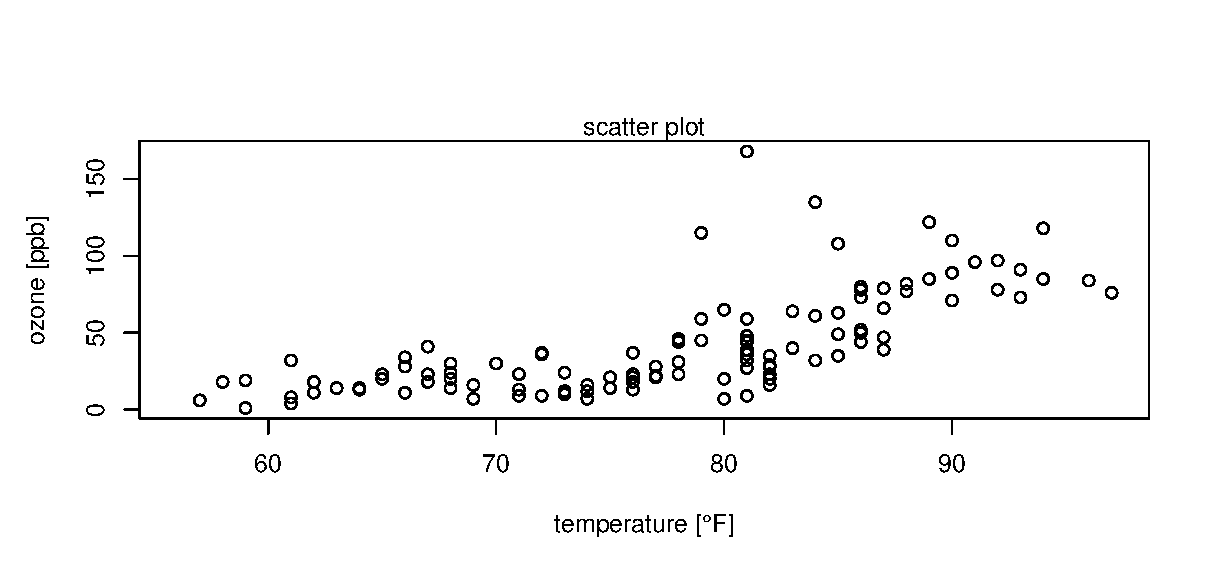
\includegraphics[scale=0.8]{scatterplot.eps}
\end{center}
\caption{Example of a scatter plot, representing the joint
distribution of measured values for the variables ``temperature''
and ``ozone'' in the \R{} data set ``airquality.'' \newline
\underline{\R:} \newline
\texttt{data("airquality")} \newline
\texttt{?airquality} \newline
\texttt{plot( airquality\$Temp , airquality\$Ozone )}}
\lb{fig:scatterplot}
\end{figure}
%

%------------------------------------------------------------------
\subsection[Sample covariance]{Sample covariance}
\lb{subsec:covar}
%------------------------------------------------------------------
The first standard measure describing degree of association in the 
joint distribution for a metrically scaled two-dimensional 
variable~$(X,Y)$ is the dimensionful \textbf{sample covariance} 
$s_{XY}$ (metr), defined by

\begin{itemize}
\item[(i)] From a raw data set:
%
\begin{eqnarray}
\lb{eq:covar}
s_{XY}
& := & \frac{1}{n-1}\left[\,(x_{1}-\bar{x})(y_{1}-\bar{y})+\ldots
+ (x_{n}-\bar{x})(y_{n}-\bar{y})\,\right]
\nonumber \\
& =: & \frac{1}{n-1}\sum_{i=1}^{n}\left(x_{i}-\bar{x}\right)
\left(y_{i}-\bar{y}\right)
\ ;
\end{eqnarray}
%
alternatively:
%
\begin{eqnarray}
\lb{eq:covar2}
s_{XY}
& = & \frac{1}{n-1}\left[\,x_{1}y_{1}+\ldots+x_{n}y_{n}
-n\bar{x}\bar{y}\,\right] \nonumber\\
& = & \frac{1}{n-1}\left[\,\sum_{i=1}^{n}x_{i}y_{i}
-n\bar{x}\bar{y}\,\right] \ .
\end{eqnarray}
%

\item[(ii)] From a relative frequency distribution:
%
\begin{eqnarray}
s_{XY}
& := & \frac{n}{n-1}\left[\,(a_{1}-\bar{x})(b_{1}-\bar{y})h_{11}
+ \ldots + (a_{k}-\bar{x})(b_{l}-\bar{y})h_{kl}
\,\right] \nonumber\\
& =: & \frac{n}{n-1}\sum_{i=1}^{k}\sum_{j=1}^{l}
\left(a_{i}-\bar{x}\right)\left(b_{j}-\bar{y}\right)h_{ij} \ ;
\end{eqnarray}
%
alternatively:
%
\begin{eqnarray}
\lb{eq:covarrelfreq2}
s_{XY}
& = & \frac{n}{n-1}\left[\,a_{1}b_{1}h_{11}+\ldots
+a_{k}b_{l}h_{kl}-\bar{x}\bar{y}\,\right] \nonumber \\
& = & \frac{n}{n-1}\left[\,\sum_{i=1}^{k}\sum_{j=1}^{l}
a_{i}b_{j}h_{ij}-\bar{x}\bar{y}\,\right] \ .
\end{eqnarray}
%
\end{itemize}
%
\underline{\textbf{Remark:}} The alternative formulae provided here 
prove computationally more efficient.

\medskip
\noindent
\underline{\R:} \texttt{cov(\textit{variable1},
\textit{variable2})} \\
\underline{EXCEL, OpenOffice:} \texttt{COVARIANCE.S} (dt.:
\texttt{KOVARIANZ.S, KOVAR})

\vspace{5mm}
\noindent
In view of its defining equation~(\ref{eq:covar}), the sample 
covariance can be given the following geometrical interpretation. 
For a total of $n$ data points $(x_{i},y_{i})$, it quantitfies the 
degree of excess of \textit{signed} rectangular areas 
$\left(x_{i}-\bar{x}\right)\left(y_{i}-\bar{y}\right)$ with 
respect to the common \textbf{centroid} ${\displaystyle 
\boldsymbol{r}_{C}:=\left(\begin{array}{c}
\bar{x} \\ \bar{y} \end{array}\right)}$ of the $n$~data points in 
favour of either positive or negative signed areas, if 
any.\footnote{The centroid is the special case of equal mass 
points, with masses ${\displaystyle m_{i}=\frac{1}{n}}$, of the 
centre of gravity of a system of $n$ discrete massive objects, 
defined by 
${\displaystyle\boldsymbol{r}_{C}:=\frac{\sum_{i=1}^{n}m_{i}
\boldsymbol{r}_{i}}{\sum_{j=1}^{n}m_{j}}}$. In two Euclidian 
dimensions the position vector is ${\displaystyle 
\boldsymbol{r}_{i}=\left(\begin{array}{c} x_{i} \\ y_{i} 
\end{array}\right)}$.}

\medskip
\noindent
It is worthwhile to point out that in the research literature it  
is standard to define for the joint distribution for a metrically 
scaled two-dimensional variable~$(X,Y)$ a dimensionful symmetric 
$\boldsymbol{(2 \times 2)}$ \textbf{sample covariance matrix} 
$\boldsymbol{S^{2}}$ according to
%
\be
\lb{eq:2dcovmat}
\boldsymbol{S^{2}} :=
\left(\begin{array}{cc}
s_{X}^{2} & s_{XY} \\
s_{XY} & s_{Y}^{2}
\end{array}\right) \ ,
\ee
%
the components of which are defined by
Eqs.~(\ref{eq:sampvardescr}) and (\ref{eq:covar}). The determinant 
of $\boldsymbol{S^{2}}$, given by
$\det(\boldsymbol{S^{2}})=s_{X}^{2}s_{Y}^{2}-s_{XY}^{2}$, is
positive as long as $s_{X}^{2}s_{Y}^{2}-s_{XY}^{2} > 0$, which
applies in most practical cases. Then $\boldsymbol{S^{2}}$ is
regular, and thus a corresponding inverse
$(\boldsymbol{S^{2}})^{-1}$ exists; cf. 
Ref.~\ct[Sec.~3.5]{hve2009}.

\medskip
\noindent
The concept of a regular sample covariance matrix
$\boldsymbol{S^{2}}$ and 
its inverse $(\boldsymbol{S^{2}})^{-1}$ generalises in a
straightforward fashion to the case of multivariate joint
distributions for metrically scaled $m$-dimensional statistical
variables~$(X,Y, \ldots, Z)$, where $\boldsymbol{S^{2}} \in
\mathbb{R}^{m \times m}$ is given by
%
\be
\lb{eq:mdcovmat}
\boldsymbol{S^{2}} :=
\left(\begin{array}{cccc}
s_{X}^{2} & s_{XY} & \ldots & s_{ZX} \\
s_{XY} & s_{Y}^{2} & \ldots & s_{YZ} \\
\vdots & \vdots & \ddots & \vdots \\
s_{ZX} & s_{YZ} & \ldots & s_{Z}^{2}
\end{array}\right) \ ,
\ee
%
and $\det(\boldsymbol{S^{2}}) \neq 0$ is required.

%------------------------------------------------------------------
\subsection[Bravais and Pearson's sample correlation 
coefficient]{Bravais and Pearson's sample correlation coefficient}
%------------------------------------------------------------------
The sample covariance $s_{XY}$ constitutes the basis for
the second standard measure characterising the joint distribution 
for a metrically scaled two-dimensional variable~$(X,Y)$ by 
descriptive means, which is the normalised and dimensionless
\textbf{sample correlation coefficient} $r$ (metr) devised by the
French physicist
\href{http://en.wikipedia.org/wiki/Auguste_Bravais}{Auguste
Bravais (1811--1863)} and the English mathematician and 
statistician
\href{http://www-history.mcs.st-and.ac.uk/Biographies/Pearson.html}{Karl
Pearson FRS (1857--1936)} for the purpose of analysing 
corresponding bivariate raw data 
$\{(x_{i},y_{i})\}_{i=1,\ldots,n}$ for the existence of a 
\textit{linear~(!!!)} statistical association. It is defined in 
terms of the bivariate sample covariance $s_{XY}$ and the 
univariate sample standard deviations $s_{X}$ and $s_{Y}$ by
(cf. Bravais (1846)~\ct{bra1846} and Pearson
(1901, 1920)~\ct{pea1901,pea1920})
%
\be
\lb{eq:correl}
\fbox{$\displaystyle
r:=\frac{s_{XY}}{s_{X}s_{Y}} \ .
$}
\ee
%
With Eq.~(\ref{eq:covar}) for $s_{XY}$, this becomes
%
\be
\lb{eq:correl2}
r = \frac{1}{n-1}\sum_{i=1}^{n}\left(\frac{x_{i}-\bar{x}}{s_{X}}
\right)\left(\frac{y_{i}-\bar{y}}{s_{Y}}\right)
= \frac{1}{n-1}\sum_{i=1}^{n}z_{i}^{X}z_{i}^{Y} \ ,
\ee
%
employing standardisation according to
Eq.~(\ref{eq:standardisationdiscriptive}) in the final step.
Due to its normalisation, the range of the sample correlation 
coefficient is $-1 \leq r \leq +1$. The sign of $r$ encodes the 
\textbf{direction} of a correlation. As to interpreting the
\textbf{strength} of a correlation via the magnitude $|r|$, in
practice one typically employs the following qualitative

\medskip
\noindent
\underline{\textbf{Rule of thumb:}}\\
$0.0 = |r|$: no correlation\\
$0.0 < |r| < 0.2$: very weak correlation\\
$0.2 \leq |r| < 0.4$: weak correlation\\
$0.4 \leq |r| < 0.6$: moderately strong correlation\\
$0.6 \leq |r| \leq 0.8$: strong correlation\\
$0.8 \leq |r| < 1.0$: very strong correlation\\
$1.0=|r|$: perfect correlation.

\medskip
\noindent
\underline{\R:} \texttt{cor(\textit{variable1},
\textit{variable2})} \\
\underline{EXCEL, OpenOffice:} \texttt{CORREL} (dt.:
\texttt{KORREL}) \\
\underline{SPSS:} Analyze $\rightarrow$ Correlate
$\rightarrow$ Bivariate \ldots: Pearson

\medskip
\noindent
In line with Eq.~(\ref{eq:2dcovmat}), it is convenient to define 
a dimensionless symmetric $\boldsymbol{(2 \times 2)}$
\textbf{sample correlation matrix} $\boldsymbol{R}$ by
%
\be
\lb{eq:2dcorrelmat}
\boldsymbol{R} :=
\left(\begin{array}{cc}
1 & r \\
r & 1
\end{array}\right) \ ,
\ee
%
which is regular and positive definite as long as its determinant 
$\det(\boldsymbol{R}) =1-r^{2}>0$. In this case, its 
inverse $\boldsymbol{R}^{-1}$ is given by
%
\be
\lb{eq:2dcorrelmatinv}
\boldsymbol{R}^{-1} =
\frac{1}{1-r^{2}}\left(\begin{array}{rr}
1 & -r \\
-r & 1
\end{array}\right) \ .
\ee
%
Note that for \textit{non-correlating} metrically scaled 
variables $X$ and $Y$, i.e., when $r=0$, the sample correlation
matrix degenerates to become a unit matrix, 
$\boldsymbol{R}=\boldsymbol{1}$.

\medskip
\noindent
Again, the concept of a regular and positive definite sample
correlation matrix $\boldsymbol{R}$, with inverse
$\boldsymbol{R}^{-1}$,
generalises to multivariate joint distributions for metrically 
scaled $m$-dimensional statistical variables~$(X,Y, \ldots, Z)$, 
where $\boldsymbol{R} \in \mathbb{R}^{m \times m}$ is given 
by\footnote{Given a data matrix $\boldsymbol{X} \in \mathbb{R}^{n 
\times m}$ for a metrically scaled $m$-dimensional statistical 
variable~$(X,Y, \ldots, Z)$, one can show that upon 
standardisation of the data according to 
Eq.~(\ref{eq:standardisationdiscriptive}), which 
amounts to a transformation $\boldsymbol{X} \mapsto \boldsymbol{Z} 
\in \mathbb{R}^{n \times m}$, the sample correlation matrix can be 
represented by 
$\displaystyle\boldsymbol{R}=\frac{1}{n-1}\,\boldsymbol{Z}^{T}
\boldsymbol{Z}$. The form of this relation is equivalent to
Eq.~(\ref{eq:correl2}).}
%
\be
\lb{eq:mdcorrelmat}
\boldsymbol{R} :=
\left(\begin{array}{cccc}
1 & r_{XY} & \ldots & r_{ZX} \\
r_{XY} & 1 & \ldots & r_{YZ} \\
\vdots & \vdots & \ddots & \vdots \\
r_{ZX} & r_{YZ} & \ldots & 1
\end{array}\right) \ ,
\ee
%
and $\det(\boldsymbol{R}) \neq 0$. Note that $\boldsymbol{R}$ is a 
dimensionless quantity which, hence, is \textbf{scale-invariant};
cf. Sec.~\ref{sec:paretodistr}.

%%%%%%%%%%%%%%%%%%%%%%%%%%%%%%%%%%%%%%%%%%%%%%%%%%%%%%%%%%%%%%%%%%%
\section[Measures of association for the ordinal scale
level]{\href{https://www.youtube.com/watch?v=6IJf7izTtjA}{Measures
of association for the ordinal scale level}}
\lb{sec:2Dord}
%%%%%%%%%%%%%%%%%%%%%%%%%%%%%%%%%%%%%%%%%%%%%%%%%%%%%%%%%%%%%%%%%%%
At the ordinal scale level, bivariate raw data 
$\{(x_{i},y_{i})\}_{i=1,\ldots,n}$ for a two-dimensional 
variable~$(X,Y)$ is not necessarily quantitative in nature. 
Therefore, in order to be in a position to define a sensible 
quantitative bivariate measure of statistical association for 
ordinal variables, one needs to introduce meaningful surrogate 
data which is numerical. This task is realised by means of 
defining so-called \textbf{rank numbers}, which are assigned to the 
original ordinal data according to the procedure described in the 
following.

\medskip
\noindent
Begin by establishing amongst the observed values 
$\{x_{i}\}_{i=1,\ldots,n}$ resp.\ $\{y_{i}\}_{i=1,\ldots,n}$ their 
natural ascending rank order, i.e.,
%
\be
\lb{eq:xyordered}
x_{(1)} \leq x_{(2)} \leq \ldots \leq x_{(n)}
\qquad\text{and}\qquad
y_{(1)} \leq y_{(2)} \leq \ldots \leq y_{(n)} \ .
\ee
%
Then, every individual $x_{i}$ resp.\ $y_{i}$ is assigned a 
\textbf{rank number} which corresponds to its position in the 
ordered sequences~(\ref{eq:xyordered}):
%
\be
x_{i} \mapsto R(x_{i}) \ , \quad
y_{i} \mapsto R(y_{i}) \ ,
\quad\quad\text{for all}\quad i=1,\ldots,n \ .
\ee
%
Should there be any ``tied ranks'' due to equality of some $x_{i}$ 
or $y_{i}$, one assigns the arithmetical mean of the corresponding 
rank numbers to all $x_{i}$ resp.\ $y_{i}$ involved in the 
``tie.'' Ultimately, by this procedure, the entire bivariate raw 
data undergoes a transformation
%
\be
\{(x_{i},y_{i})\}_{i=1,\ldots,n} \mapsto 
\{[R(x_{i}),R(y_{i})]\}_{i=1,\ldots,n} \ ,
\ee
%
yielding $n$ pairs of rank numbers to numerically represent the 
original bivariate ordinal data.

\medskip
\noindent
Given surrogate rank number data, the \textbf{means of rank
numbers} always amount to
%
\bea
\bar{R}(x) & := & \frac{1}{n}\sum_{i=1}^{n}R(x_{i})
\ = \ \frac{n+1}{2} \\
%
\bar{R}(y) & := & \frac{1}{n}\sum_{i=1}^{n}R(y_{i})
\ = \ \frac{n+1}{2} \ .
\eea
%
The \textbf{variances of rank numbers} are defined in accordance
with Eqs.~(\ref{eq:sampvardescr2}) and (\ref{eq:ssqurel2}), i.e.,
%
\bea
s_{R(x)}^{2} & := & 
\frac{1}{n-1}\,\left[\,\sum_{i=1}^{n}R^{2}(x_{i})
-n\bar{R}^{2}(x)\,\right]
\ = \ \frac{n}{n-1}\,\left[\,\sum_{i=1}^{k}R^{2}(a_{i})h_{i+}
-\bar{R}^{2}(x)\,\right] \\
%
s_{R(y)}^{2} & := & 
\frac{1}{n-1}\,\left[\,\sum_{i=1}^{n}R^{2}(y_{i})
-n\bar{R}^{2}(y)\,\right]
\ = \ \frac{n}{n-1}\,\left[\,\sum_{j=1}^{l}R^{2}(b_{j})h_{+ j}
-\bar{R}^{2}(y)\,\right] \ .
\eea
%
In addition, to characterise the joint distribution of rank 
numbers, a \textbf{sample covariance of rank numbers} is defined in 
line with Eqs.~(\ref{eq:covar2}) and (\ref{eq:covarrelfreq2}) by
%
\bea
s_{R(x)R(y)} & := & \frac{1}{n-1}\,\left[\,\sum_{i=1}^{n}
R(x_{i})R(y_{i})
-n\bar{R}(x)\bar{R}(y)\,\right] \nonumber \\
& = & \frac{n}{n-1}\,\left[\,\sum_{i=1}^{k}\sum_{j=1}^{l}
R(a_{i})R(b_{j})h_{ij} -\bar{R}(x)\bar{R}(y)\,\right] \ .
\eea
%

\vspace{5mm}
\noindent
On this fairly elaborate technical backdrop, the English 
psychologist and statistician
\href{http://en.wikipedia.org/wiki/Charles_Edward_Spearman}{Charles
Edward Spearman FRS (1863--1945)} defined a dimensionless
\textbf{sample rank correlation coefficient}~$r_{S}$ (ord), in
analogy to Eq.~(\ref{eq:correl}), by (cf. Spearman
(1904)~\ct{spe1904})
%
\be
\lb{eq:rankcorrelcoeff}
\fbox{$\displaystyle
r_{S}:=\frac{s_{R(x)R(y)}}{s_{R(x)}s_{R(y)}} \ .
$}
\ee
%
The range of this rank correlation coefficient is $-1 \leq r_{S} 
\leq +1$. Again, while the sign of $r_{S}$ encodes the 
\textbf{direction} of a rank correlation, in interpreting the
\textbf{strength} of a rank correlation via the magnitude $|r_{S}|$
one usually employs the qualitative

\medskip
\noindent
\underline{\textbf{Rule of thumb:}}\\
$0.0 = |r_{S}|$: no rank correlation\\
$0.0 < |r_{S}| < 0.2$: very weak rank correlation\\
$0.2 \leq |r_{S}| < 0.4$: weak rank correlation\\
$0.4 \leq |r_{S}| < 0.6$: moderately strong rank correlation\\
$0.6 \leq |r_{S}| \leq 0.8$: strong rank correlation\\
$0.8 \leq |r_{S}| < 1.0$: very strong rank correlation\\
$1.0=|r_{S}|$: perfect rank correlation.

\medskip
\noindent
\underline{\R:} \texttt{cor(\textit{variable1},
\textit{variable2}, method = "spearman")} \\
\underline{SPSS:} Analyze $\rightarrow$ Correlate
$\rightarrow$ Bivariate \ldots: Spearman

\medskip
\noindent
When \textit{no tied ranks} occur, Eq.~(\ref{eq:rankcorrelcoeff})
simplifies to (cf. Hartung \textit{et al} 
(2005)~\ct[p~554]{haretal2005})
%
\be
r_{S}=1-\frac{6\sum_{i=1}^{n}[R(x_{i})-R(y_{i})]^{2}}{n(n^{2}-1)}
\ .
\ee
%

%%%%%%%%%%%%%%%%%%%%%%%%%%%%%%%%%%%%%%%%%%%%%%%%%%%%%%%%%%%%%%%%%%%
\section[Measures of association for the nominal scale
level]{Measures of association for the nominal scale level}
\lb{sec:2Dnom}
%%%%%%%%%%%%%%%%%%%%%%%%%%%%%%%%%%%%%%%%%%%%%%%%%%%%%%%%%%%%%%%%%%%
Lastly, let us turn to consider the case of quantifying 
the degree of statistical association in bivariate raw data 
$\{(x_{i},y_{i})\}_{i=1,\ldots,n}$ for a nominally scaled 
two-dimensional variable~$(X,Y)$, with categories 
$\{(a_{i},b_{j})\}_{i=1,\ldots,k;j=1,\ldots,l}$. The starting 
point are the observed bivariate \textbf{absolute}
resp.\ \textbf{relative (cell) frequencies} $o_{ij}$ and $h_{ij}$
of the joint distribution for $(X,Y)$, with univariate
\textbf{marginal frequencies} $o_{i+}$ resp.\ $h_{i+}$ for $X$ and
$o_{+ j}$ resp.\ $h_{+ j}$ for $Y$. The
\textbf{$\boldsymbol{\chi}^{2}$--statistic} 
devised by the English mathematical statistician 
\href{http://www-history.mcs.st-and.ac.uk/Biographies/Pearson.html}{Karl
Pearson FRS (1857--1936)} rests on the notion of statistical 
independence of two one-dimensional variables $X$ and $Y$ in that 
it takes the corresponding formal condition provided by 
Eq.~(\ref{eq:statindep}) as a reference state. A simple algebraic 
manipulation of this condition obtains 
%
\be
h_{ij} = h_{i+}h_{+j}
\quad\Rightarrow\quad
\frac{o_{ij}}{n} = \frac{o_{i +}}{n}\,\frac{o_{+ j}}{n}
\quad\overbrace{\Rightarrow}^{\text{multiplication by}\ n}\quad
o_{ij} = \frac{o_{i +}o_{+ j}}{n} \ .
\ee
%
Pearson's descriptive $\chi^{2}$--statistic (cf. Pearson 
(1900)~\ct{pea1900}) is then defined by
%
\be
\fbox{$\displaystyle
\chi^{2} := \sum_{i=1}^{k}\sum_{j=1}^{l}\frac{\left(o_{ij}
-{\displaystyle\frac{o_{i+}o_{+ 
j}}{n}}\right)^{2}}{{\displaystyle\frac{o_{i+}
o_{+ j}}{n}}}
= n\sum_{i=1}^{k}\sum_{j=1}^{l}\frac{\left(h_{ij}
-h_{i+}h_{+ j}\right)^{2}}{h_{i+}h_{+ j}} \ ,
$}
\ee
%
whose range of values amounts to $0 \leq \chi^{2} \leq 
\max(\chi^{2})$, with $\max(\chi^{2}):=n\,[\min(k,l)-1]$.

\medskip
\noindent
\underline{\textbf{Remark:}} Provided $\displaystyle 
\frac{o_{i+}o_{+j}}{n} \geq 5$ for all $i=1, \ldots, k$ and $j=1, 
\ldots, l$, Pearson's $\chi^{2}$--statistic can be employed for 
the analysis of statistical associations amongst the components of 
a two-dimensional variable~$(X,Y)$ of almost all combinations of 
scale levels.

\medskip
\noindent
The problem with Pearson's $\chi^{2}$--statistic is that, due to 
its variable spectrum of values, it is not immediately clear how 
to use it efficiently in interpreting the \textbf{strength} of 
statistical associations. This shortcoming can, however, be 
overcome by resorting to the \textbf{measure of association}
proposed by the Swedish mathematician, actuary, and statistician 
\href{http://www-history.mcs.st-and.ac.uk/Biographies/Cramer_Harald.html}{Carl
Harald Cram\'{e}r (1893--1985)}, which basically is the 
result of a special kind of normalisation of Pearson's measure. 
Thus, \textbf{Cram\'{e}r's $\boldsymbol{V}$}, as it has come to be 
known, is defined by (cf. Cram\'{e}r (1946)~\ct{cra1946})
%\ct[p~282]{cra1946})
%
\be
\lb{eq:cramv}
\fbox{$\displaystyle
V:=\sqrt{\frac{\chi^{2}}{\max(\chi^{2})}} \ ,
$}
\ee
%
with range $0 \leq V \leq 1$. For the interpretation of the 
strength of statistical association in the joint distribution for a 
two-dimensional categorical variable~$(X,Y)$, one may thus employ 
the qualitative

\medskip
\noindent
\underline{\textbf{Rule of thumb:}}\\
$0.0 \leq V < 0.2$: weak association\\
$0.2 \leq V < 0.6$: moderately strong association\\
$0.6 \leq V \leq 1.0$: strong association.

\medskip
\noindent
\underline{\R:} \texttt{assocstats(\textit{contingency table})}
(package: \texttt{vcd}, by Meyer \textit{et al}
(2017)~\ct{meyetal2017}) \\
\underline{SPSS:} Analyze $\rightarrow$ Descriptive Statistics
$\rightarrow$ Crosstabs \ldots $\rightarrow$ Statistics \ldots:
Chi-square, Phi and Cramer's V

%%%%%%%%%%%%%%%%%%%%%%%%%%%%%%%%%%%%%%%%%%%%%%%%%%%%%%%%%%%%%%%%%%%
%%%%%%%%%%%%%%%%%%%%%%%%%%%%%%%%%%%%%%%%%%%%%%%%%%%%%%%%%%%%%%%%%%%
